\renewcommand{\theequation}{\theenumi}
\begin{enumerate}[label=\arabic*.,ref=\thesubsection.\theenumi]
\numberwithin{equation}{enumi}
\item Without drawing a figure, determine whether the points $\myvec{-1\\2}$, $\myvec{0\\0}$, $\myvec{3\\-4}$ lie outside, on the circumference, or inside the circle
\begin{align}
\vec{x}^T\vec{x}+\myvec{-5 & 2}\vec{x}-5 = 0
\end{align}
\solution
Without drawing a figure, determine whether
the points \myvec{-1\\2} , \myvec{0\\0} , \myvec{3\\-4}  lie outside, on the
circumference, or inside the circle
\begin{align}
    \vec{x}^T\vec{x}+ \myvec{-5 & 2}\vec{x}-5 = 0 \label{eq:solutions/4/2/1/eq1}
\end{align}
The equation of circle with center $\vec{c}$ can be expressed as
\begin{align}
    \vec{x}^T\vec{x}-2\vec{c}^T\vec{x}+f = 0 \label{eq:solutions/4/2/1/eq2}
\end{align}
Comparing \eqref{eq:solutions/4/2/1/eq2} with \eqref{eq:solutions/4/2/1/eq1}
\begin{align}
\vec{c}=\myvec{\frac{5}{2} \\ -1},f=-5 \\
 r=\sqrt{\norm{\vec{c}}^2-f} = \sqrt{\frac{49}{4}}
\end{align}
\begin{enumerate}
\item
Let a= \myvec{-1\\2}
\begin{align}
\norm{\vec{a-c}}=\sqrt{\frac{49}{4}+9}=\sqrt{\frac{84}{4}}
\implies \norm{\vec{a-c}}>r 
\end{align}
Point a is outside the circle
\item
Let b= \myvec{0\\0}
\begin{align}
\norm{\vec{b-c}}=\sqrt{\frac{25}{4}+1}=\sqrt{\frac{29}{4}}
\implies \norm{\vec{a-c}}<r 
\end{align}
Point b is inside the circle.
\item
Let d= \myvec{3\\-4}
\begin{align}
\norm{\vec{d-c}}=\sqrt{\frac{1}{4}+9}=\sqrt{\frac{37}{4}}
\implies \norm{\vec{d-c}}<r 
\end{align}
Point d is inside the circle.
\end{enumerate}
\begin{figure}[!ht]
\centering
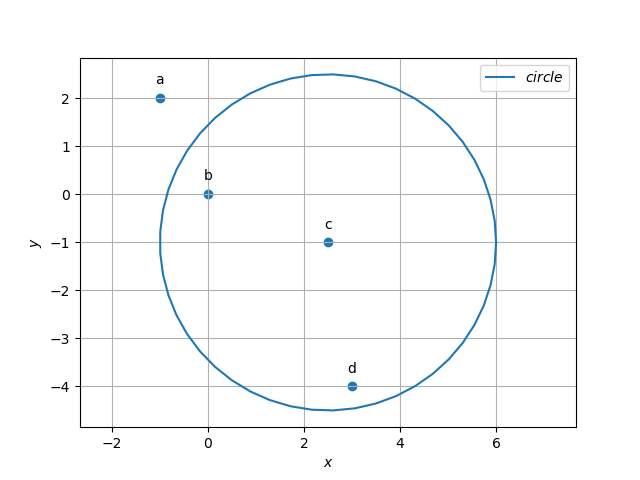
\includegraphics[width=\columnwidth]{./solutions/4/2/1/assign4}
\caption{Points a,b,d in the circle with center c}
\label{eq:solutions/4/2/1/Fig:1}
\end{figure}



\item Find the points of intersection of the line
\begin{align}
    \label{eq:solutions/4/2/2/eq1}\myvec{3 & 2}\vec x = 12
\end{align}
and the circle
\begin{align}
    \label{eq:solutions/4/2/2/eq:circle} \norm{\vec{x}}^2 = 13
\end{align}
and for what values of $c$ the line
\begin{align}
    \label{eq:solutions/4/2/2/tangent}\myvec{3 &2}\vec x = c 
\end{align}
touches the circle.
\\
%
\solution
If $\vec P$ be a point on the line and $\vec n$ is the normal vector, the equation of the line can be expressed as 
\begin{align}
    & \vec n^T\brak{\vec x - \vec P}=0\\
    & \label{eq:solutions/4/2/2/eq2}\implies \vec n^T \vec x = c
\end{align}
where
\begin{align}
    c= \vec n^T \vec P
\end{align}
From \brak{\ref{eq:solutions/4/2/2/eq1}} and \brak{\ref{eq:solutions/4/2/2/eq2}}, 
\begin{align}
     \vec n^T = \myvec{3 & 2}
\end{align}
We know,
\begin{align}
    &\vec m^T \vec n = 0\\
    &\implies \vec m^T \myvec{3 \\2} = 0\\
    &\implies \vec m ^T = \myvec{-2 & 3}
\end{align}

Now,
\begin{align}
    &\vec n^T \vec P = c \\
    &\implies \myvec{3 & 2} \vec P= 12
\end{align}

$\vec P$ can be
\begin{align}
    \myvec{4\\0}, \myvec{2\\3}, \myvec{0\\6}
\end{align}
Let us take 
\begin{align}
    \vec P =\myvec{2\\3}=\vec q
\end{align}
The circle equation:
\begin{align}
    \vec x^T \vec x + 2 \vec u^T\vec x +f=0
\end{align}
From \brak{\ref{eq:solutions/4/2/2/eq:circle}},
\begin{align}
    &\vec u=\myvec{0\\0}\\
    & f=-13
\end{align}
The points of intersection of the line
\begin{align}
    L: \vec x = \vec q + \mu \vec m \quad ,\mu \in \mathbb R
\end{align}
with the conic section
\begin{align}
    \vec x^T \vec V \vec x +2\vec u^T \vec x+ f=0
\end{align}
are given by 
\begin{align}
    \label{eq:solutions/4/2/2/points of intersection}\vec x_i = \vec q + \mu _i \vec m
\end{align}
where,

\begin{multline}
\mu_i = \frac{1}
{
\vec{m}^T\vec{V}\vec{m}
}
\lbrak{-\vec{m}^T\brak{\vec{V}\vec{q}+\vec{u}}}
\\
\pm
{\small
\rbrak{\sqrt{
\sbrak{
\vec{m}^T\brak{\vec{V}\vec{q}+\vec{u}}
}^2
-
\brak
{
\vec{q}^T\vec{V}\vec{q} + 2\vec{u}^T\vec{q} +f
}
\brak{\vec{m}^T\vec{V}\vec{m}}
}
}
}
\end{multline}
For circle,
\begin{align}
    &\vec V = \vec I\\ 
    & \therefore \mu_i = \frac{1}{13}\lbrak{-5 \pm \rbrak{\sqrt{25- \brak{13-13}13}
    }
    }\\
    & = \frac{1}{13}\brak{-5 \pm 5}\\
    & = 0, -\frac{10}{13}
\end{align}
Using \brak{\ref{eq:solutions/4/2/2/points of intersection}}, the points of intersection are given by
\begin{align}
    \vec x = \myvec{2\\3} , \myvec{\frac{46}{13}\\ \frac{9}{13}}
\end{align}
Points of contact are given by
\begin{align}
    \vec q = \vec V^{-1} \brak{\kappa \vec n - \vec u}\\
    \kappa = \pm \sqrt{\frac{\vec u^T \vec V^{-1} \vec u -f}{\vec n^T \vec V^{-1} \vec n}}
\end{align}
Since for circle,
\begin{align}
    &\vec V= \vec I\\
    &\therefore \vec V^{-1} = \vec I \quad \because \vec I^{-1}
    = \vec I\\
    &\therefore \kappa =\pm  \sqrt{\frac{-f}{\vec n^T \vec n}}\quad\because \vec u^T\vec u= 0\\
    & = \pm \sqrt{\frac{13}{\myvec{3 & 2}\myvec{3\\2}}}\\
    & = \pm \sqrt{\frac{13}{13}}\\
    & = \pm 1\\
    &\therefore \vec q = \pm 1\myvec{3\\2}\\
    & = \myvec{3\\2}, \myvec{-3\\-2}
\end{align}
From \brak{\ref{eq:solutions/4/2/2/tangent}},
\begin{align}
    c = \myvec{3 & 2}\myvec{3\\2} = 13, \\ \myvec{3&2}\myvec{-3\\-2}=-13
\end{align}
The line \brak{\ref{eq:solutions/4/2/2/tangent}} touches the circle for $c = 13, -13$.

\begin{figure}[!ht]
\centering
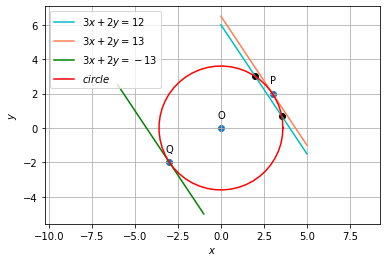
\includegraphics[width=1\columnwidth]{./solutions/4/2/2/figure.png}
\caption{Circle with tangent and intersection lines}
\label{eq:solutions/4/2/2/}
\end{figure}


%
\item Prove that the line 
\begin{align}
\myvec{3 &2}\vec{x}=30 \label{eq:solutions/4/2/3/given_line_eq}
\end{align}
touches the circle
\begin{align}
\vec{x}^T\vec{x}-\myvec{10 & 2}\vec{x}+13 = 0 \label{eq:solutions/4/2/3/given_circle_eq}
\end{align}
and find the coordinates of the point of contact.
%
\solution


The vector equation of a line can be expressed as 
\begin{align}
    \vec{x} = \vec{q} +\mu\vec{m} \label{eq:solutions/4/2/3/vec_eqn_of_line}
\end{align}
The general equation of a second degree can be expressed as :
\begin{align}
\vec{x}^T\vec{V}\vec{x}+2\vec{u}^T\vec{x}+f=0\label{eq:solutions/4/2/3/gen__quad_eqn}
\end{align}


  %  \begin{figure}[!ht]
    %\centering
    %\resizebox{\columnwidth}{!}{\input{Assignment_4_figure}}
    %\caption{$\triangle{ABC}$ with $AD$ as median and $AM \perp BC$}
    %\label{eq:solutions/4/2/3/fig:triangle}
   % \end{figure}

Comparing \eqref{eq:solutions/4/2/3/given_circle_eq} with \eqref{eq:solutions/4/2/3/gen__quad_eqn}
\begin{align}
\vec{u}=\myvec{-5 \\ -1}, f=13 
\end{align}
If $\vec{n}$ is the normal vector of a line, equation of that line can be written as 
\begin{align}
\vec{n}^T\vec{x} = c \label{eq:solutions/4/2/3/eq1}
\end{align}
Comparing \eqref{eq:solutions/4/2/3/given_line_eq} with \eqref{eq:solutions/4/2/3/eq1}
\begin{align}
\vec{n} = \myvec{3 \\ 2}\label{eq:solutions/4/2/3/eq2}
\end{align}
 The point of contact $\vec{q}$, of a line with a normal vector $\vec{n}$ to the conic in \eqref{eq:solutions/4/2/3/gen__quad_eqn} is given by:
\begin{align}
\vec{q} = \vec{V}^{-1}\brak{\kappa \vec{n}-\vec{u}} 
%\label{eq:solutions/4/2/3/eq3} 
\\
\kappa = \pm \sqrt{\frac{\vec{u}^T\vec{V}^{-1}\vec{u}-f}{\vec{n}^T\vec{V}^{-1}\vec{n}}} \label{eq:solutions/4/2/3/eq4}
\end{align}
We know that, for a circle, 
\begin{align}
\vec{V} = \vec{I}  
\end{align}
and from the properties of an Identity matrix, 
\begin{align}
\vec{I}^{-1} &= \vec{I} \\
\vec{I}\vec{X} &= \vec{X}   
\end{align}
Solving for the point of contact using the above equations we get,
\begin{align}
\kappa &= \pm \sqrt{\frac{\myvec{ -5 & -1 }\myvec{-5 \\ -1} - 13}{\myvec{3 & 2 }\myvec{3 \\ 2 }}} \\
&= \pm \sqrt{\frac{26 - 13}{13}} \\
& =  \pm \sqrt{1} \\
q &= \myvec{3 \\2 } - \myvec{-5 \\ -1} \\
&= \myvec{8 \\ 3}
\end{align}
If the line in \eqref{eq:solutions/4/2/3/vec_eqn_of_line} touches  \eqref{eq:solutions/4/2/3/gen__quad_eqn} at exactly one point $\vec{q}$, then 
\begin{align}
\vec{m}^T\brak{\vec{V}\vec{q}+\vec{u}} = 0 \label{eq:solutions/4/2/3/eq3}
\end{align}
It can seen that for the given line
\begin{align}
\vec{m} = \myvec{1 \\ -1.5} 
\end{align}
Solving \eqref{eq:solutions/4/2/3/eq3} for given line and circle, we get
\begin{align}
&= \myvec{1 & -1.5}\brak{\myvec{8 \\ 3}+\myvec{-5 \\ -1}} \\
&= \myvec{1 & -1.5}\myvec{3 \\ 2}\\
&= 0
\end{align}
Hence, it is proved that the given line touches the given circle at only one point and so it is a tangent.
\begin{figure}[!ht]
\centering
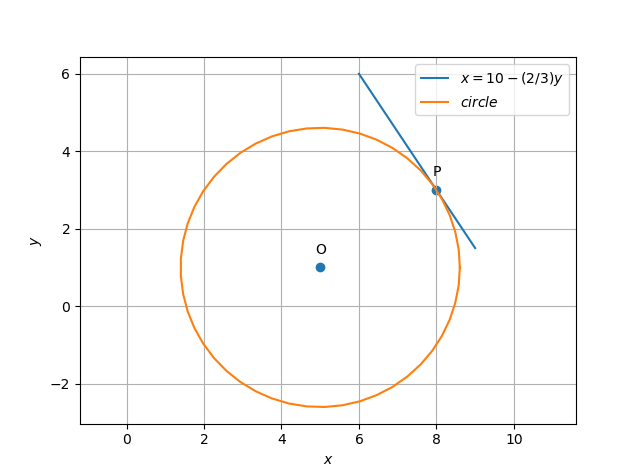
\includegraphics[width=\columnwidth]{./solutions/4/2/3/assignment_5_fig.png}
\caption{Circle with center (5 1) and having the line (3 2)x =30 as tangent with (8 3) as point of contact.}
\label{eq:solutions/4/2/3/Fig:Circle}
\end{figure}

\item For what values of $m$ does the line 
\begin{align}
\myvec{m &-1}\vec{x}=0
\label{eq:solutions/4/2/4/1.1}
\end{align}
touch the circle
\begin{align}
\vec{x}^T\vec{x}-\myvec{6 & 2}\vec{x}+8 = 0 \label{eq:solutions/4/2/4/1.2}
\end{align}
\solution
The general equation of a circle is 
\begin{align}
\implies \vec{x}^T\vec{x}+ 2\vec{u}^T\vec{x} + f = 0 \label{eq:solutions/4/2/4/2.1}
\end{align}
\begin{align}
\text{If $r$ is radius,} f =\vec{u}^T\vec{u}-r^2  \label{eq:solutions/4/2/4/2.2} \\  
  \text{center }\vec{c} =-\vec{u}
\end{align}
From equations \ref{eq:solutions/4/2/4/1.2} and \ref{eq:solutions/4/2/4/2.1},
\begin{align}
 \vec{u}  = \myvec{-3 \\ -1}\\
\implies \text{Center of the cirlce } \vec{c} = \myvec{3 \\ 1}
\end{align}
Also, radius can be determined as follows from \ref{eq:solutions/4/2/4/2.2}
\begin{align}
  \implies 8=\myvec{-3&-1}\myvec{-3\\-1}-r^2\\
  \implies 8=10 -r^2\\
  \implies r=\sqrt{2}
\end{align}
Given equation of the line is
\begin{align}
\myvec{m&-1}\vec{x}&=0 
\end{align}

It can be expressed as:-
\begin{align}
L: \quad \vec{x} = \vec{q} + \mu \vec{m} \quad \mu \in \mathbb{R} \label{eq:solutions/4/2/4/2.10} \\
\end{align}
The normal vector to the line is obtained as
\begin{align}
\vec{n} = \vec{q} + \vec{u}\\
\implies \vec{q}  = \vec{n} -  \vec{u}\\
\vec{n} =\myvec{m & -1 }^T  \text{ and } \vec{u} =\myvec{-3 & -1}^T\\
\vec{q} = \myvec{m+3 \\ 0}
\end{align}
The point $\vec{q}$ also satisfies the equation of the circle at \ref{eq:solutions/4/2/4/1.2}.
\begin{align}
\vec{q}^T\vec{q}+ 2\vec{u}^T\vec{q} + f = 0 \\
%\vec{q}^T\vec{q}-\myvec{6 &  2}\vec{q}+8 = 0 
\end{align}
\begin{multline}
(\vec{n} -\vec{ u})^T(\vec{n} -\vec{ u})+2\vec{u}^T(\vec{n} -\vec{ u})\\+f = 0
\end{multline}
\begin{multline}
\norm{\vec{n}}^2 - \vec{n}^T \vec{u} - \vec{u}^T\vec{n} + \norm{\vec{u}}^2  + 2\vec{u}^T\vec{n}\\ -2 \norm{\vec{u}}^2 +f = 0 
\end{multline}
\begin{multline}
\norm{\vec{n}}^2 - \vec{n}^T \vec{u} +\vec{n}^T\vec{u} - \norm{\vec{u}}^2  +f = 0 
\end{multline}
\begin{align}
\norm{\vec{n}}^2 - \norm{\vec{u}}^2  +f = 0\\ 
(m^2 +1) - 10 +8 = 0 \\
m^2 -1 =0\\
m=\pm 1
\end{align}
For the line \ref{eq:solutions/4/2/4/1.1} to be a tangent to circle at equation \ref{eq:solutions/4/2/4/1.2}, the values of $m$ are $\pm1$
\begin{figure}[!]
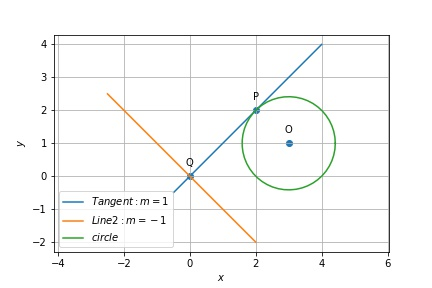
\includegraphics[width=1\columnwidth]{./solutions/4/2/4/CircleTangent.jpg}
\caption{Circle with tangent}
\label{eq:solutions/4/2/4/}
\end{figure}



\renewcommand{\theequation}{\theenumi}
\item Prove that the circle 
\begin{align}
\vec{x}^T\vec{x}-2a\myvec{1 & 1}\vec{x}+a^2 = 0
\label{eq:solutions/4/2/5/eq1}
\end{align}
touches the coordinate axes.
\solution
Let r be the radius of the circle. Now for proving that the circle touches the co-ordinate axes we have to prove that it touches x axis and y axes at points such that:
\begin{align}
\vec{Point_{1}} = \myvec{ r \\ 0 \\}\label{eq:solutions/4/2/5/eq B}
\end{align}
\begin{align}
\vec{Point_{2}} = \myvec{ 0 \\ r \\} \label{eq:solutions/4/2/5/eq C}
\end{align}
The general equation of a circle is given by
\begin{align}
\vec{x}^T\vec{x} - 2\vec{O}^T\vec{x} + \vec{f}  &= 0 \label{eq:solutions/4/2/5/eq 2}
\end{align}
Where $\vec{O}$ is the centre and $\vec{r}$ is the radius of the circle.\\
Substituting \eqref{eq:solutions/4/2/5/eq B} in \eqref{eq:solutions/4/2/5/eq1}, we rewrite \eqref{eq:solutions/4/2/5/eq1}as:
\begin{align}
\myvec{r&0}\myvec{r\\0}-2\myvec{a & a}\myvec{r\\0}+\vec{a}^2 = 0 \label{eq:solutions/4/2/5/eq3}
\end{align}
\begin {align}
\implies\vec{r}^2 -2\left(\vec{a}\vec{r}\right)+\vec{a}^2=0
\end{align}
\begin {align}
\implies\vec{r}^2 -2\left(\vec{a}\vec{r}\right)+\vec{a}^2=0
\end{align}
\begin {align}
\implies\left(\vec{r}- \vec{a}\right)^2=0
\end{align}
\begin{align}
\implies\vec{r}= \vec{a}
\end{align}
Similarly, substituting \eqref{eq:solutions/4/2/5/eq C} in \eqref{eq:solutions/4/2/5/eq1}, we rewrite \eqref{eq:solutions/4/2/5/eq1}as:
\begin{align}
\myvec{0&r}\myvec{0\\r}-2\myvec{a & a}\myvec{0\\r}+\vec{a}^2 = 0 
%\label{eq:solutions/4/2/5/eq3}
\end{align}
\begin {align}
\implies\vec{r}^2 -2\left(\vec{a}\vec{r}\right)+\vec{a}^2=0
\end{align}
\begin {align}
\implies\vec{r}^2 -2\left(\vec{a}\vec{r}\right)+\vec{a}^2=0
\end{align}
\begin {align}
\implies\left(\vec{r}- \vec{a}\right)^2=0
\end{align}
\begin{align}
\implies\vec{r}= \vec{a}
\end{align}
Therefore, the circle touches x axis at $\vec{Point_{1}}$ i.e $\myvec{ a \\ 0}$ and y axis at $\vec{Point_{2}}$ i.e $\myvec{ 0\\ a}$ \\
Hence,it is proved that the circle touches the co-ordinate axes
\begin{figure}[h!]
\centering
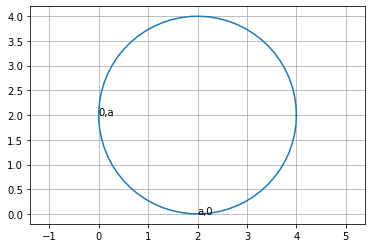
\includegraphics[width=\columnwidth]{./solutions/4/2/5/circle new.png}
\caption{Circle touching the co-ordinate axes \\a=2}
\label{eq:solutions/4/2/5/}
\end{figure}

\item Show that two circles can be drawn to pass through the point $\myvec{1\\2}$ and touch the coordinate axes, and find their equations.
\solution
Let us consider  we have a circle which passes through the point   $ \myvec { 1 \\ 2 \\	} $  and touches  x - axis at point  $ \myvec { r \\ 0 \\	} $ and y - axis  at $ \myvec { 0 \\ r \\ } $. Radius of the circle is $\vec{r}$ since it touches both axes. Hence we have 3 points which are :
\begin{align}
\vec{P_{1}} = \myvec{ 1 \\ 2 \\}
\end{align}
\begin{align}
\vec{p_{2}} = \myvec{ r \\ 0 \\}
\end{align}
\begin{align}
\vec{P_{3}} = \myvec{ 0 \\ r \\} \label{eq:solutions/4/2/6/2.3}
\end{align}

The general equation of circle is :
\begin{align}
\norm{\vec{x} - \vec{O}} = r
\end{align}

Substituting the given coordinates:
\begin{align}
\norm{  \vec{P_2} - \vec{O}}^{2} = r^{2} \label{eq:solutions/4/2/6/2.5}
\end{align}

\begin{align}
\norm{  \vec{ P_3} - \vec{O}}^{2} = r^{2} \label{eq:solutions/4/2/6/2.6}
\end{align}


\begin{align}
\norm{  \vec{ P_1} - \vec{O}}^{2} = r^{2} \label{eq:solutions/4/2/6/2.7}
\end{align}

From equation \ref{eq:solutions/4/2/6/2.5}, \ref{eq:solutions/4/2/6/2.6} and \ref{eq:solutions/4/2/6/2.7} we have 
%
%\begin{align}
%\norm{  \myvec{ r \\ 0 \\} - \vec{O}}^{2}  - \norm{ \myvec{ 1 \\ 2 \\}  - \vec{O}}^{2}   = 0 \label{eq:solutions/4/2/6/2.8}
%\end{align}
%
%\begin{align}
%\norm{ \myvec{ 0 \\ r \\} - \vec{O}}^{2}   - \norm{\myvec{ 1 \\ 2 \\} - \vec{O}}^{2}  = 0 \label{eq:solutions/4/2/6/2.9}
%\end{align}




\begin{align}
\norm{  \vec{ P_2} - \vec{O}}^{2}  - \norm{ \vec{P_1}  - \vec{O}}^{2}   = 0 \label{eq:solutions/4/2/6/2.8}
\end{align}
And,
\begin{align}
\norm{ \vec{ P_3} - \vec{O}}^{2}   - \norm{\vec{ P_1} - \vec{O}}^{2}  = 0 \label{eq:solutions/4/2/6/2.9}
\end{align}

 Simplifying   \ref{eq:solutions/4/2/6/2.8} and \ref{eq:solutions/4/2/6/2.9},
\begin{align}
\myvec{\vec{P_2} - \vec{O}}^T \myvec{\vec{P_2} - \vec{ O}} - \myvec{\vec{P_1} - \vec{O}}^T\myvec{\vec{P_1} - \vec{O}} = \vec{0} \label{eq:solutions/4/2/6/2.10}
\end{align}



\begin{align}
\implies \norm{\vec{P_2}}^2 - 2 \vec{P_2}^T\vec{O} - \norm{\vec{P_1}}^2 +2\vec{P_1}^T \vec{O}  = \vec{0} \label{eq:solutions/4/2/6/2.11}
\end{align}

 Substituting the value of $\norm{\vec{P_1}}$ and $\norm{\vec{P_2}}$ and other values then rearranging it, we get :
\begin{align}
\myvec{2 -2r & 4 \\}\myvec{O} = 5-r^2 \label{eq:solutions/4/2/6/2.12}
\end{align}





Similarly,

\begin{align}
\myvec{\vec{P_3} - \vec{O}}^T \myvec{\vec{P_3} - \vec{ O}} - \myvec{\vec{P_1} - \vec{O}}^T\myvec{\vec{P_1} - \vec{O}} = \vec{0} \label{eq:solutions/4/2/6/2.13}
\end{align}



\begin{align}
\implies \norm{\vec{P_3}}^2 - 2 \vec{P_3}^T\vec{O} - \norm{\vec{P_1}}^2 +2\vec{P_1}^T \vec{O}  = \vec{0} \label{eq:solutions/4/2/6/2.14}
\end{align}
Substituting the value of $\norm{\vec{P_1}}$ and $\norm{\vec{P_3}}$ and other values then  rearranging it, we get :

\begin{align}
\myvec{2  & 4 -2r \\}\myvec{O} = 5-r^2 \label{eq:solutions/4/2/6/2.15}
\end{align}















Combining \ref{eq:solutions/4/2/6/2.15} and \ref{eq:solutions/4/2/6/2.12}

\begin{align}
\myvec{2 - 2r  &  4 \\   2 & 4 - 2r \\} \myvec{O} = \myvec{5 - r^2 \\ 5 - r^2 \\} \label{eq:solutions/4/2/6/2.17}
\end{align}
Transforming the matrix into row-echelon form \\
\begin{align}
\myvec{2 - 2r  &  4 &  5 - r^2 \\   2 & 4 - 2r &  5 - r^2 \\}  \label{eq:solutions/4/2/6/2.18}
\end{align}

	\begin{align}
\myvec{
	2 - 2r & 4 & 5 - r^2 \\
	2 & 4 - 2r & 5 - r^2 \\
}
\xleftrightarrow[]{R1 \leftarrow \frac{R1}{2 - 2r} } \nonumber  \\
%
\myvec{
	1 & \frac{-2}{r-1} & \frac{r^2 - }{2\left( r - 1\right)} \\
	2 & 4 - 2r & 5 - r^2\\
}
\xleftrightarrow[]{R2 \leftarrow  R2 - 2R1 } \nonumber  \\
%
\myvec{
	1 & \frac{-2}{r - 1} & \frac{r^2 - 5}{2 \left( r - 1 \right)} \\
	0 & \frac{2r\left(r - 3 \right) }{ r - 1} & \frac{r \left(r^2 - 5 \right)}{r - 1}
}
\xleftrightarrow[]{R2 \leftarrow \left( \frac{1 - r}{ 2r \left( r - 3\right)}\right)R2 } \nonumber  \\
%	
\myvec{
	1 & \frac{-2}{r - 1} & \frac{r^2 - 5}{2 \left(r - 1\right)} \\
	0 & 1 & \frac{r^2 - 5}{2 \left(r - 3\right)}
}
\xleftrightarrow[]{R1 \leftarrow  R1 - \left( \frac{-2}{r - 1} \right)R2 } \nonumber   \\
\myvec{
	1 & 0 & \frac{r^2 - 5}{2 \left(r - 3\right)} \\
	0 & 1 & \frac{r^2 - 5}{2 \left(r - 3\right)}
}
\end{align}
So,
\begin{align}
\vec{O} = \myvec{ \frac{r^2 - 5}{2 \left(r - 3\right)} \\ \frac{r^2 - 5}{2 \left(r - 3\right)} \\} \label{eq:solutions/4/2/6/2.19}
\end{align}



Now subsituting the \ref{eq:solutions/4/2/6/2.3} in \ref{eq:solutions/4/2/6/2.7}, we have
\begin{align}
\norm{  \vec{ P_3} - \vec{O}}^{2} = r^{2} \label{eq:solutions/4/2/6/2.20}
\end{align}

Subsituting the value of $\vec{O}$ in \ref{eq:solutions/4/2/6/2.7} and simplify,
\begin{align}
\myvec{\vec{P_3} - \vec{O}}^T\myvec{\vec{P_3} - \vec{O}} = r^2 \label{eq:solutions/4/2/6/2.21}
\end{align}


\begin{align}
 \implies \norm{\vec{P_3}}^2 - \vec{P_3}^T\vec{O}  -  \vec{P_3} \vec{O}^T +\norm{\vec{O}}^2 = r^2 \label{eq:solutions/4/2/6/2.22.1}
\end{align}
Putting the values  of $\vec{O}$ from \ref{eq:solutions/4/2/6/2.19} and $\norm{\vec{P_3}}^2$

\begin{align}
\implies - \vec{P_3}^T\vec{O}  -  \vec{P_3} \vec{O}^T    = -  \norm{\vec{O}}^2 \label{eq:solutions/4/2/6/2.22.22}
\end{align}



\begin{align}
\implies - \myvec{0 \\ r}^T\myvec{ \frac{r^2 - 5}{2 \left(r - 3\right)} \\ \frac{r^2 - 5}{2 \left(r - 3\right)} \\}  -  \myvec{0 \\ r} \myvec{ \frac{r^2 - 5}{2 \left(r - 3\right)} \\ \frac{r^2 - 5}{2 \left(r - 3\right)} \\}^T    = -  \norm{\vec{O}}^2 \label{eq:solutions/4/2/6/2.22.2}
\end{align}

Subsituting the value of $\norm{\vec{O}}^2$ and simplify it,
\begin{align}
\implies 2r \left( \frac{r^2 - 5}{2 \left(r - 3\right)} \right) = 2 \left( \frac{r^2 - 5}{2 \left(r - 3\right)} \right)^2 
\end{align}




\begin{figure}[htb!]	
	\centering	
	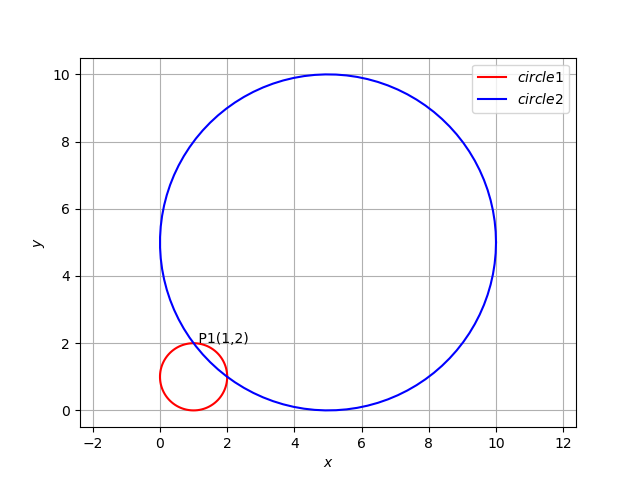
\includegraphics[width=\columnwidth]{./solutions/4/2/6/Circle.png}	
	\caption{Two circles passing through a common point}
	\label{eq:solutions/4/2/6/fig1}	
\end{figure}

\begin{align}
 \implies r  =  \frac{r^2 - 5}{2 \left(r - 3\right)} 
\end{align}


\begin{align}
\implies r^2 - 6r +5 = 0
\end{align}


\begin{align}
\implies \left( r -1\right) \left( r- 5\right) = 0
\end{align}

\begin{align}
\implies r = 1, r = 5.
\end{align}

Hence,
\begin{align}
\vec{O_1} = \myvec{5 \\ 5 \\} \text{and,}  \vec{O_2} = \myvec{1 \\ 1 \\}
\end{align}

Hence equation of circles are :
\begin{align}
\norm{\vec{x} - \myvec{5 \\ 5 \\}} = 5
\end{align}
And,
\begin{align}
\norm{\vec{x} - \myvec{1 \\ 1 \\}} = 1
\end{align}


\item Find the length of the tangent from the point $\myvec{7\\4}$ to the circle
\begin{align}
		 \vec{x}^T\vec{x}- \myvec{4 & 6}\vec{x}+12=0\label{eq:solutions/4/2/7/eq:1}
\end{align}
\solution

The general equation of a second degree can be expressed as :
\begin{align}
	\vec{x}^T\vec{V}\vec{x}+2\vec{u}^T\vec{x}+f=0\label{eq:solutions/4/2/7/gen__quad_eqn}
\end{align}
Let the equation of the tangent be
\begin{align}
	\myvec{-m & 1}\vec{x}=c \label{eq:solutions/4/2/7/given_line_eq}
\end{align}

We know that, for a circle, 
\begin{align}
	\vec{V} = \vec{I}  \\
	\vec{c} = -\vec{u}
\end{align}
Comparing the equation \eqref{eq:solutions/4/2/7/eq:1} and \eqref{eq:solutions/4/2/7/gen__quad_eqn}
we get
\begin{align}
	\vec{u}&=\myvec{-2 \\ -3}, f=12 \\
	\vec{c}&=\myvec{2 \\ 3}
\end{align} 

The normal vector to the line is obtained as 
\begin{align}
	\vec{n} = \vec{q} + \vec{u} \label{eq:solutions/4/2/7/eq1}\\
	\vec{q} = \vec{n} - \vec{u}
\end{align}

Comparing the equation \eqref{eq:solutions/4/2/7/given_line_eq} 
\begin{align}
	\vec{n} &= \myvec{-m &1}^T
\end{align}
Given
\begin{align}
	 \vec{u}&=\myvec{-2 \\ -3}\\
\implies	 \vec{q} &= \myvec{-m+2 \\ 4}\label{eq:solutions/4/2/7/eq:2}
\end{align}
The point q also satisfies the equation of the circle at \eqref{eq:solutions/4/2/7/gen__quad_eqn}
\begin{align}
	\vec{q}^T\vec{q}+2\vec{u}^T\vec{q}+f=0\\
	(\vec{n} -\vec{u})^T(\vec{n} -\vec{u})+2\vec{u}^T(\vec{n} -\vec{u}) +f =0\\
	\norm{\vec{n}}^2 - \vec{n}^T\vec{u}-\vec{u}^T\vec{n}+\norm{\vec{u}}^2+2\vec{u}^T\vec{n}- 2\norm{\vec{u}}^2+f=0\\
	\norm{\vec{n}}^2 -\norm{\vec{u}}^2+f=0\\
	m^2+1-13+12=0\\
	m^2=0\\
	m=0\label{eq:solutions/4/2/7/eq:3}
\end{align}
Simplying \eqref{eq:solutions/4/2/7/eq:3} and \eqref{eq:solutions/4/2/7/eq:2} we get
\begin{align}
	\vec{q} &= \myvec{2 \\ 4}
\end{align}

Let $\vec{p} =\myvec{7 \\ 4}$
The length of tangent is 
\begin{align}
	\norm{\vec{p}-\vec{q}}&= \sqrt{(7-2)^2 + (4-4)^2}\\
	&=\sqrt{25}\\
	&=5
\end{align}
\begin{figure}[!htbp]
 	\centering
 	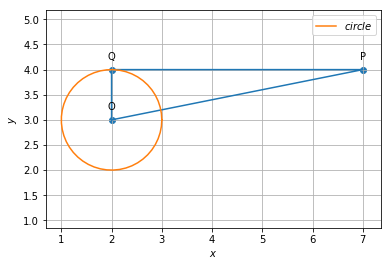
\includegraphics[width =\columnwidth]{./solutions/4/2/7/circle.png}
 	\caption{Perpendicular Line }
 	\label{eq:solutions/4/2/7/fig:1}
\end{figure}	


\numberwithin{equation}{enumi}
\item  Find the equations of tangents to the circle 
\begin{align}
\vec{x}^T\vec{x}-\myvec{4 & 3}\vec{x}+5 = 0 \label{eq:solutions/4/2/8/given_circle_eq}
\end{align}
that are parallel to the line
\begin{align}
\myvec{1 &1}\vec{x}=0 \label{eq:solutions/4/2/8/given_line_eq}
\end{align}
%
\solution
The vector equation of a line can be expressed as 
\begin{align}
    \vec{x} = \vec{q} +\mu\vec{m} \label{eq:solutions/4/2/8/vec_eqn_of_line}
\end{align}
The general equation of a second degree can be expressed as :
\begin{align}
\vec{x}^T\vec{V}\vec{x}+2\vec{u}^T\vec{x}+f=0\label{eq:solutions/4/2/8/gen__quad_eqn}
\end{align}

Comparing \eqref{eq:solutions/4/2/8/given_circle_eq} with \eqref{eq:solutions/4/2/8/gen__quad_eqn}
\begin{align}
\vec{u}=\myvec{-2 \\ \frac{-3}{2}}, f=5
\end{align}
If $\vec{n}$ is the normal vector of a line, equation of that line can be written as 
\begin{align}
\vec{n}^T\vec{x} = c \label{eq:solutions/4/2/8/eq1}
\end{align}
Comparing \eqref{eq:solutions/4/2/8/given_line_eq} with \eqref{eq:solutions/4/2/8/eq1}
\begin{align}
\vec{n} = \myvec{1 \\ 1}\label{eq:solutions/4/2/8/eq2}
\end{align}
Since it is mentioned that the tangent is parallel to given line it will have same normal vector. \\
 The point of contact $\vec{q}$, of a line with a normal vector $\vec{n}$ to the conic in \eqref{eq:solutions/4/2/8/gen__quad_eqn} is given by:
\begin{align}
\vec{q} = \vec{V}^{-1}\brak{\kappa \vec{n}-\vec{u}} \label{eq:solutions/4/2/8/eq3} \\
\kappa = \pm \sqrt{\frac{\vec{u}^T\vec{V}^{-1}\vec{u}-f}{\vec{n}^T\vec{V}^{-1}\vec{n}}} \label{eq:solutions/4/2/8/eq4}
\end{align}
The point of contact $\vec{q}$, of a line with a normal vector $\vec{n}$ to the conic in \eqref{eq:solutions/4/2/8/gen__quad_eqn} is given by:
\begin{align}
\vec{q} = \vec{V}^{-1}\brak{\kappa \vec{n}-\vec{u}} 
%\label{eq:solutions/4/2/8/eq3}
 \\
\kappa = \pm \sqrt{\frac{\vec{u}^T\vec{V}^{-1}\vec{u}-f}{\vec{n}^T\vec{V}^{-1}\vec{n}}} 
%\label{eq:solutions/4/2/8/eq4}
\end{align}
We know that, for a circle, 
\begin{align}
\vec{V} = \vec{I}  
\end{align}
and from the properties of an Identity matrix, 
\begin{align}
\vec{I}^{-1} &= \vec{I} \\
\vec{I}\vec{X} &= \vec{X}   
\end{align}
Solving for the point of contact using the above equations we get,
\begin{align}
\kappa &= \pm \sqrt{\frac{\myvec{ -2 & -1.5 }\myvec{-2 \\ -1.5} - 5}{\myvec{1 & 1 }\myvec{1 \\ 1 }}} \\
&= \pm \sqrt{\frac{6.25 - 5}{2}} \\
& =  \pm \sqrt{\frac{5}{8}}\\
\end{align}
So there are two tangents to a circle which are parallel to given line which touch circle at two different points  $\vec{q_1}$ and $\vec{q_2}$
\begin{align}
\vec{q_1} &= \myvec{\sqrt{\frac{5}{8}} \\ \sqrt{\frac{5}{8}}} + \myvec{2 \\ \frac{3}{2}} \\
&= \myvec{\frac{279}{100} \\ \frac{229}{100}}
\end{align}
\begin{align}
\vec{q_2} &= \myvec{-\sqrt{\frac{5}{8}} \\ \sqrt{\frac{5}{8}}} + \myvec{2 \\ \frac{3}{2}} \\
&= \myvec{\frac{121}{100} \\ \frac{71}{100}}
\end{align}
Since points $\vec{q_1}$ and $\vec{q_2}$ lie on tangent they satisfy the line equation of tangents, there are two different tangents with same normal vector
\begin{align}
\vec{n}^T\vec{q_1} = c_1 
%\label{eq:solutions/4/2/8/eq1}
\end{align}
\begin{align}
\vec{n}^T\vec{q_2} = c_2 
%\label{eq:solutions/4/2/8/eq1}
\end{align}
$c_1$ and $c_2$ are some constants
\begin{align}
c_1=\myvec{1 & 1}\myvec{\frac{279}{100} \\ \frac{229}{100}}\newline
&= \frac{127}{25}
\end{align}
\newline
\begin{align}
c_2=\myvec{\frac{121}{100} \\ \frac{71}{100}}\newline
&= \frac{48}{25}
\end{align}
So line equations of tangents to the given circle which are parallel to line are
\begin{align}
\myvec{1 &1}\vec{x}=\frac{127}{25}
\end{align}and
\newline
\begin{align}
\myvec{1 &1}\vec{x}=\frac{48}{25}
\end{align}
%
\begin{figure}[]
\centering
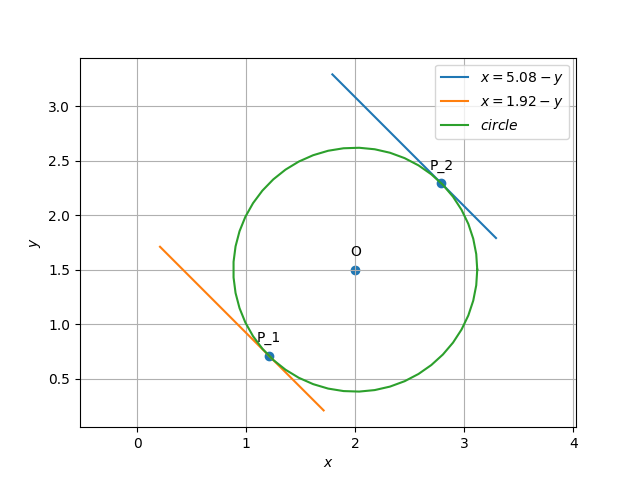
\includegraphics[width=\columnwidth]{./solutions/4/2/8/Figure_1.png}
\caption{Circle with center (2 1.5) and having the lines (1 1)x =5.08 and (1 1)x =1.92 as tangents with (2.79 2.29) and (1.21 0.71) as point of contact.}
\label{eq:solutions/4/2/8/Fig:Circle}
\end{figure}


\renewcommand{\theequation}{\theenumi}
\item Find the equations of the tangents to the circle
\begin{align}
\vec{x}^T\vec{x}-\myvec{7 & 5}\vec{x}+18 = 0
\end{align}
at the points $\myvec{4\\3}$ and $\myvec{3\\2}$, showing that they are parallel.
\\
\solution

The general equation of a second degree can be expressed as: 
\begin{align}
   \vec{x}^T\vec{V}\vec{x}+2\vec{u}^T\vec{x}+f=0
\end{align}
Comparing 1.0.1 with 2.0.1
\begin{align}
  \vec{V}=\vec{I}, \vec{u}=\myvec{\frac{-7}{2}\\\frac{-5}{2}}, f=18
\end{align}
The vector equation of a line can be expressed as  
\begin{align}
\vec{x}=\vec{q}+ \mu \vec{m}
\end{align}
{Tangent-1} Given point
\begin{align}
\vec{q_1}=\myvec{4\\3}
\end{align}
The direction vector of the line joining the point $\vec{q_1}$ and the centre $\vec{c}$ expressed as:
\begin{align}
 \vec{n_1}=\vec{q_1}-\vec{c}
 \end{align}
\begin{align}
\implies \vec{n_1}=\vec{q_1}+\vec{u}      
\end{align}
where, 
\begin{align}
\vec{c}=-\vec{u} 
\end{align}
The vector $\vec{n_1}$ is normal to the tangent drawn at $\vec{q_1}$. 
From (2.0.2) and (2.1.1) we get,
\begin{align}
\vec{n_1}^T=\myvec{\frac{1}{2} & \frac{1}{2}}
\end{align}
We know,
\begin{align}
\vec{m}^T\vec{n_1} = 0
\end{align}
\begin{align}
\implies \vec{m}^T\myvec{\frac{1}{2}\\ \frac{1}{2}} = 0
\end{align}
\begin{align}
\implies \vec{m}^T= \myvec{\frac{-1}{2} & \frac{1}{2}}
\end{align}
If $\vec{q_1}$ be a point on the line and $\vec{n_1}$ is the normal vector then
the equation of the line can be expressed From(2.0.3) is :
\begin{align}
 \vec{n_1}^T (\vec{x}-\vec{q_1})=0
\end{align}
\begin{align}
 \implies \vec{n_1}^T \vec{x}= c
\end{align}
where
\begin{align}
 c=\vec{n_1}^T \vec{q_1}
\end{align}
Using the equations (2.1.1) and (2.1.5),
\begin{align}
 \implies c=\myvec{\frac{1}{2} & \frac{1}{2}} \myvec{4\\3}= \frac{7}{2}
\end{align}
From (2.1.10), Line equation of Tangent-1 is:
\begin{align}
 \myvec{\frac{1}{2} & \frac{1}{2}} \vec{x}= \frac{7}{2}
\end{align}
\begin{align}
  \implies \boxed{\myvec{1 & 1} \vec{x}= 7}
\end{align}
{Tangent-2} Now,
\begin{align}
\vec{q_2}=\myvec{3\\2}
\end{align}
The direction vector of the line joining the point $\vec{q_2}$ and the centre $\vec{c}$ expressed as:
\begin{align}
 \vec{n_2}=\vec{q_2}-\vec{c}
 \end{align}
 \begin{align}
 \implies \vec{n_2}=\vec{q_2}+\vec{u}
 \end{align}
 where, 
\begin{align}
\vec{c}=-\vec{u} 
\end{align}
The vector $\vec{n_2}$ is normal to the tangent drawn at $\vec{q_2}$.
From (2.0.2) and (2.2.1),
\begin{align}
\vec{n_2}^T=\myvec{\frac{-1}{2} & \frac{-1}{2}}
\end{align}
We know,
\begin{align}
\vec{m}^T\vec{n_2} = 0
\end{align}
\begin{align}
\implies \vec{m}^T\myvec{\frac{-1}{2}\\ \frac{-1}{2}} = 0
\end{align}
\begin{align}
\implies \vec{m}^T= \myvec{\frac{1}{2} & \frac{-1}{2}}
\end{align}
If $\vec{q_2}$ be a point on the line and $\vec{n_2}$ is the normal vector, the equation of the line can be expressed From (2.0.3) is:
\begin{align}
 \vec{n_2}^T (\vec{x}-\vec{q_2})=0
\end{align}
\begin{align}
 \implies \vec{n_2}^T \vec{x}= c
\end{align}
where
\begin{align}
 c=\vec{n_2}^T \vec{q_2}
\end{align}
Using the equations 2.2.1 and 2.2.5,
\begin{align}
 \implies c=\myvec{\frac{-1}{2} & \frac{-1}{2}} \myvec{3\\2}= \frac{-5}{2}
\end{align}
From (2.2.10), Line equation of Tangent-2 is:
\begin{align}
 \myvec{\frac{-1}{2} & \frac{-1}{2}} \vec{x}= \frac{-5}{2}
\end{align}
\begin{align}
  \implies \boxed {\myvec{1 & 1} \vec{x}= 5 }
\end{align}
{Result}
From the equations (2.1.14) and (2.2.14), normal vectors of Tangent-1 and Tangent-2 are equal. \newline 
\centering Hence, the two tangents are parallel.
\begin{figure}[h!]
	\centering
	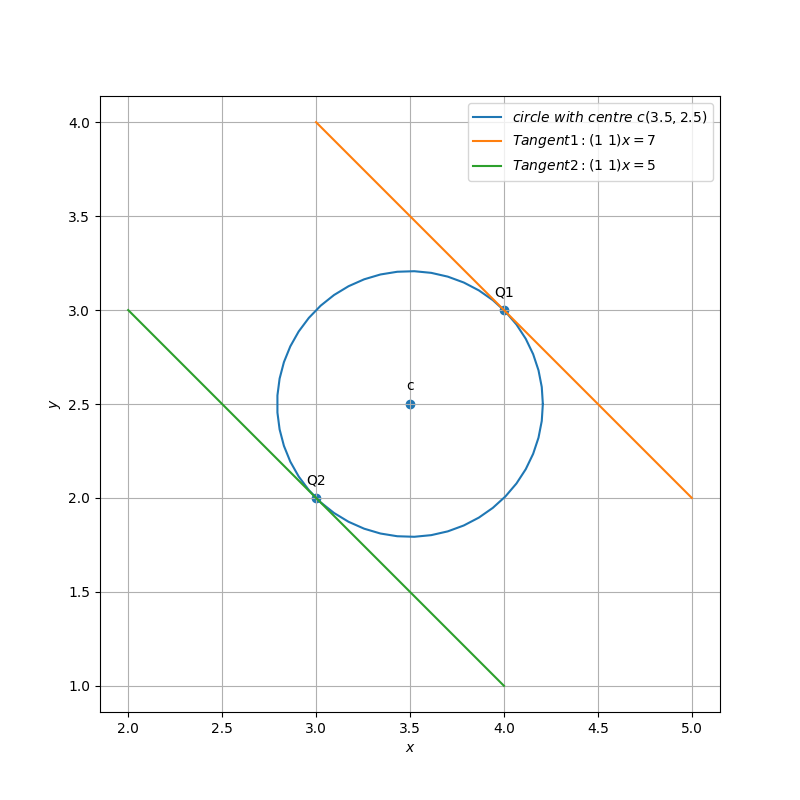
\includegraphics[width=\columnwidth]{./solutions/4/2/9/Codes/A4.png}
	\caption{Tangents to the circle at given points}
	\label{eq:solutions/4/2/9/myfig}
\end{figure}

\item Find the equations of the tangent and normal to the circle
\begin{align}
\vec{x}^T\vec{x}+\myvec{-6 & 4}\vec{x}-12 = 0
\end{align}
at the point $\myvec{6\\2}$.
\numberwithin{equation}{enumi}
\item Prove that the line
\begin{align}
\myvec{1 & 1}\vec{x} = 1 \label{eq:solutions/4/2/11eq:1}
\end{align}
touches the circle
\begin{align}
\vec{x^T}\vec{x} - \myvec{8 & 6}\vec{x} + 7 = 0 \label{eq:solutions/4/2/11eq:2}    
\end{align}
and find the equations of the parallel and perpendicular tangents.
%
\\
\solution
The general equation of a second degree can be expressed as,
\begin{align}
\vec{x^T}\vec{V}\vec{x} + 2\vec{u^T}\vec{x} + f = 0 \label{eq:solutions/4/2/11eq:3}
\end{align}
Comparing \eqref{eq:solutions/4/2/11eq:2} and \eqref{eq:solutions/4/2/11eq:3} we get,
\begin{align}
\vec{u} = \myvec{-4 \\ -3} \label{eq:solutions/4/2/11eq:4}
\end{align}
\begin{align}
f = 7 \label{eq:solutions/4/2/11eq:5}    
\end{align}
If $\vec{n}$ is the normal vector, $\vec{P}$ is a point on that line then equation of the line can be written as,
\begin{align}
\vec{n^T}\brak{\vec{x-P}} = 0\\
\implies \vec{n^Tx} = c \label{eq:solutions/4/2/11eq:7}
\end{align}
 where c = $\vec{n^TP}$.
Comparing \eqref{eq:solutions/4/2/11eq:1} and \eqref{eq:solutions/4/2/11eq:7} we get,
\begin{align}
\vec{n} = \myvec{1 \\ 1} and \ c = 1 \label{eq:solutions/4/2/11eq:8}
\end{align}\\
The point of contact q, of a line with a normal vector $\vec{n}$ to the conic in \eqref{eq:solutions/4/2/11eq:3} is given by,
\begin{align}
\vec{q} = \vec{V^{-1}}\brak{\kappa\vec{n} - \vec{u}} \label{eq:solutions/4/2/11eq:9}
\end{align}
\begin{align}
\kappa = \pm \sqrt{\frac{\vec{u^TV^{-1}u}-f}{\vec{n^TV^{-1}n}}} \label{eq:solutions/4/2/11eq:10}
\end{align}\\
For a circle,
\begin{align}
\vec{V} = \vec{I} \label{eq:solutions/4/2/11eq:11}
\end{align}
where I is the Identity matrix..
Solving for $\kappa$ using \eqref{eq:solutions/4/2/11eq:10} we get,
\begin{align}
\kappa = \pm 3 \label{eq:solutions/4/2/11eq:12}
\end{align}
\begin{align}
i.e. \ \vec{q_1} = \myvec{1 \\ 0} \ for \ \kappa = -3 \label{eq:solutions/4/2/11eq:13}
\end{align}
and
\begin{align}
\vec{q_2} = \myvec{7 \\ 6} \ for \ \kappa = 3 \label{eq:solutions/4/2/11eq:14}
\end{align}
To prove that the line touches the circle at $\vec{q}$ need to check that
\begin{align}
\vec{m^T}\brak{\vec{V}\vec{q}+\vec{u}} = 0 \label{eq:solutions/4/2/11eq:15}
\end{align}
We know that,
\begin{align}
\vec{m^T}\vec{n} = 0 \label{eq:solutions/4/2/11eq:16}
\end{align}
\begin{align}
\implies m = \myvec{$-$1 \\ 1} \label{eq:solutions/4/2/11eq:17} 
\end{align}\\
Using \eqref{eq:solutions/4/2/11eq:13}, \eqref{eq:solutions/4/2/11eq:14} and \eqref{eq:solutions/4/2/11eq:17}, the expression in \eqref{eq:solutions/4/2/11eq:15} holds true for both $\vec{q_1}$ and $\vec{q_2}$ which means that both those points lie on the circle i.e. there will be a tangent passing through each of them which can be found out using \eqref{eq:solutions/4/2/11eq:7}
\begin{align}
i.e. \ \vec{n^T}\vec{q_1} = c_1 \label{eq:solutions/4/2/11eq:18}
\end{align}
\begin{align}
\vec{n^T}\vec{q_2} = c_2 \label{eq:solutions/4/2/11eq:19}
\end{align}
where,
\begin{align}
c_1 = \vec{n^Tq_1} = \myvec{1 & 1}\myvec{1 \\ 0} = 1  \label{eq:solutions/4/2/11eq:20}
\end{align}
which was already obtained in \eqref{eq:solutions/4/2/11eq:8} and\\
\begin{align}
c_2 = \vec{n^Tq_2} = \myvec{1 & 1}\myvec{7 \\ 6} = 13 \label{eq:solutions/4/2/11eq:21}
\end{align}
Using \eqref{eq:solutions/4/2/11eq:18} the given line in the question is obtained which is \eqref{eq:solutions/4/2/11eq:1}.
Therefore, the tangent parallel to \eqref{eq:solutions/4/2/11eq:1} is,
\begin{align}
\myvec{1 & 1}\vec{x} = 13 \label{eq:solutions/4/2/11eq:22}
\end{align}\\
And the line(s) perpendicular to \eqref{eq:solutions/4/2/11eq:1} can be found out using \eqref{eq:solutions/4/2/11eq:8} and here the normal vector for this line will be $\vec{m}$ which was calculated using \eqref{eq:solutions/4/2/11eq:17} and its equation(s) will be,
\begin{align}
    \vec{m^Tx} = c_3 \label{eq:solutions/4/2/11eq:23}
\end{align}
\begin{align}
    \vec{m^Tx} = c_4 \label{eq:solutions/4/2/11eq:24}
\end{align}
where,
\begin{align}
c_3 = \vec{m^Tq_1} = \myvec{-1 & 1}\myvec{1 \\ 0} = -1 \label{eq:solutions/4/2/11eq:25}
\end{align}
\begin{align}
c_4 = \vec{m^Tq_2} =  \myvec{-1 & 1}\myvec{7 \\ 6} = -1  \label{eq:solutions/4/2/11eq:26}
\end{align}\\
Therefore, the line perpendicular to \eqref{eq:solutions/4/2/11eq:1} and also to \eqref{eq:solutions/4/2/11eq:22} is,
\begin{align}
 \myvec{-1 & 1}\vec{x} = -1 \label{eq:solutions/4/2/11eq:27}   
\end{align}

In Fig. \ref{eq:solutions/4/2/11Fig.1}. $\vec{C}$ is the center of the circle. $\vec{q_1}$ and $\vec{q_2}$ are points of contact with the circle. 
\begin{figure}[!ht]
\centering
    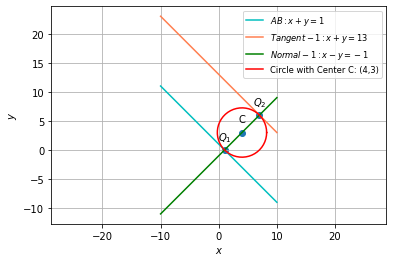
\includegraphics[width=\columnwidth]{./solutions/4/2/11/Figure.png}
    \caption{Tangents and Normal on the Circle}
    \label{eq:solutions/4/2/11Fig.1}
\end{figure}
\\
Line 1 is \eqref{eq:solutions/4/2/11eq:1}, Line 2 is \eqref{eq:solutions/4/2/11eq:22} and Line 3 is \eqref{eq:solutions/4/2/11eq:27}.

\renewcommand{\theequation}{\theenumi}
\item Find the equation of the tangent at the origin to the circle
\begin{align}
\vec{x}^T\vec{x}+2\myvec{g & f}\vec{x} = 0
\end{align}
\numberwithin{equation}{enumi}
%
\item Prove that the line 
\begin{align}
\myvec{\cos\alpha &\sin\alpha}\vec{x} = p
\end{align}
touches the circle
\begin{align}
\norm{\vec{x}-\myvec{a\\b}}=r
\end{align}
if
\begin{align}
r = \pm \brak{p-a\cos\alpha-b\sin\alpha}
\end{align}
\renewcommand{\theequation}{\theenumi}
\item Find the points of contact of the tangents to the circle
\begin{align}
\norm{\vec{x}}=5
\end{align}
that pass through the point $\myvec{7\\1}$ and write down the equations of the tangents.
\numberwithin{equation}{enumi}

\item Prove that the tangent to the circle 
\begin{align}
\norm{\vec{x}}^2=5
\end{align}
at the point $\myvec{1\\-2}$ also touches the circle
\begin{align}
\vec{x}^T\vec{x}+\myvec{-8 & 6}\vec{x}+20 = 0
\end{align}
and find the coordinates of the point of contact.
\item Find the equations of the circles that touch the lines
\begin{align}
\myvec{0 & 1}\vec{x} &= 0
\\
\myvec{0 & 1}\vec{x} &= 4
\\
\myvec{2 & 1}\vec{x} &= 2
\end{align}
\item Find the coordinates of the middle point of the chord
\begin{align}
\myvec{1 & 7}\vec{x} &= 25
\end{align}
of the circle
\begin{align}
\norm{\vec{x}}=5
\end{align}
\renewcommand{\theequation}{\theenumi}
\item Find the equation of the chord of the circle
\begin{align}
\vec{x}^T\vec{x}-\myvec{6 & 4}\vec{x}-23 = 0
\end{align}
which has the point $\myvec{4\\1}$ as its middle point.
\item Prove that the circle
\begin{align}
\vec{x}^T\vec{x}-\myvec{6 & 4}\vec{x}+9 = 0
\end{align}
subtends an angle $\tan^{-1}\frac{12}{5}$ at the origin.
\numberwithin{equation}{enumi}
\item Find the condition that the line
\begin{align}
\myvec{l & m}\vec{x} + n &= 0
\end{align}
should touch the circle
\begin{align}
\norm{\vec{x}-\myvec{a\\b}}=r
\end{align}
\renewcommand{\theequation}{\theenumi}
\item Verify that the perpendicular bisector of the chord joining two points $\vec{x}_1, \vec{x}_2$ on the circle
\begin{align}
\vec{x}^T\vec{x}+2\myvec{g & f}\vec{x} + c = 0
\end{align}
passes through the centre.
\end{enumerate}
